\documentclass[a4paper,12pt]{article}
\usepackage[utf8]{inputenc}
\usepackage[T1]{fontenc}

\usepackage[left=1.5cm, right=1.5cm, top=2cm, bottom=2cm, twoside]{geometry}

\usepackage{esvect}
\usepackage{siunitx}
\usepackage{fancybox}

\usepackage{amsmath}
\usepackage{amsfonts}
\usepackage{amssymb}
\usepackage{amsthm}

\usepackage{braket}
\usepackage{graphicx}
%\usepackage{mathptmx}
\usepackage{newtxtext}
\usepackage{newtxmath}
%\usepackage{tikz}
\usepackage{pgfplots}
\usepackage{siunitx}
\usepackage{hyperref}


\usepackage{pstricks}
\usepackage{pstricks-add}
\usepackage{pst-plot}
\pgfplotsset{compat=1.17}

\usepackage[french]{babel}
%Raccourcis de la flemme
\newcommand{\R}{\mathbb{R}}
%\newcommand{\C}{\mathbb{C}}
\newcommand{\D}{\, \mbox{d}}

\hypersetup{
 pdfauthor={Tanneguy Blandin},
 pdftitle={Devoir maison: Physique du solide},
 pdfkeywords={},
 pdfsubject={},
 pdfcreator={Me}, 
 pdflang={French}}

%Définition des numéros d'éxercices
\newcounter{numExo}
\newcounter{partExo}
\newcounter{numQuestion}
\newcounter{numSubQuestion}


\newcommand{\exercice}[1]{%
  \stepcounter{numExo}%
  \setcounter{partExo}{0}%
  \setcounter{numQuestion}{0}%
  \setcounter{numSubQuestion}{0}%
    \noindent
    \section*{Exercice \arabic{numExo}: #1}
    \addcontentsline{toc}{section}{\protect\numberline{}Exercice \arabic{numExo}: #1}
}
\newcommand{\partexo}[1]{%
  \stepcounter{partExo}%
    \setcounter{numQuestion}{0}%
    \setcounter{numSubQuestion}{0}%
    \noindent
    \subsection*{\Alph{partExo} -- #1}
    \addcontentsline{toc}{subsection}{\protect\numberline{}\Alph{partExo}: #1}
    }

\newcommand{\Question}{%
  \stepcounter{numQuestion}%
  \setcounter{numSubQuestion}{0}%
 \par\noindent \textbf{\arabic{numQuestion}.\hspace{2pt}}}


\newenvironment{question}%
{%
\ttfamily %
  \stepcounter{numQuestion}%
  \setcounter{numSubQuestion}{0}%
 \par\noindent \textbf{\arabic{numQuestion}}
}%
{%
\normalfont\par
}

\newenvironment{info}%
{%
\ttfamily %
}%
{%
\normalfont
}

\newcommand{\subquestion}{%
  \stepcounter{numSubQuestion}%
  \par{}\hspace{3pt}\textbf{\alph{numSubQuestion}.\hspace{2pt}}}


%%INFO DOC
\title{Devoir maison \\ Physique des matériaux \\ \large{\textsc{insa} Rennes -- 3 SGM}}
\date{Mars 2021}
\author{Tanneguy Blandin}

  
\begin{document}
\maketitle


\exercice{Cristal bidimensionnel}

\partexo{Réseau}

\begin{figure}[htb]
  \centering
  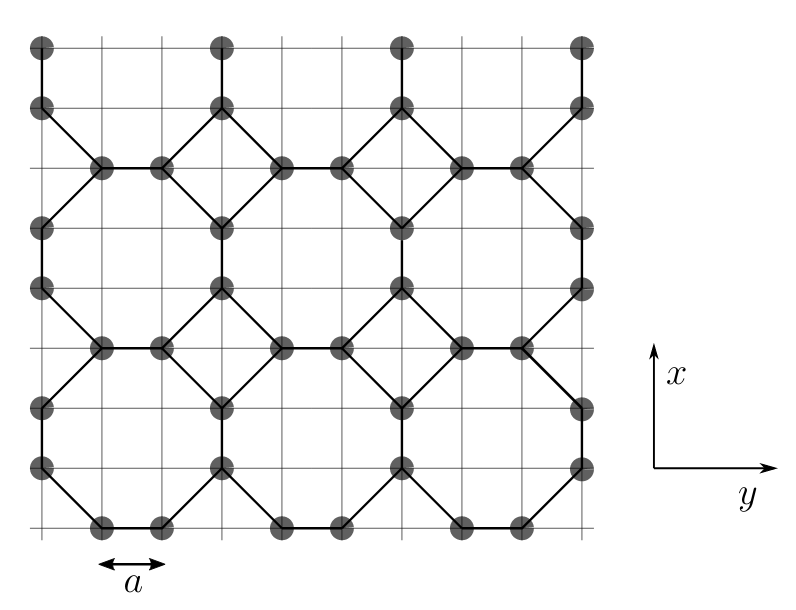
\includegraphics[width=0.5\textwidth]{./pictures/cristal2D.png}
  \caption{Cristal 2D}
  \label{fig:cristal2D}
\end{figure}

\begin{question}
  Donner les coordonnées des vecteurs $(\vv{a},\vv{b})$ qui définissent une maille primitive de ce réseau dans le repère $Oxy$ orthonormé, en fonction de $a_0$.
\end{question}

La maille est une maille carrée, les vecteurs de la maille élémentaire de ce réseau sont $\vv{a}=(3a_0,0)$ et $\vv{b}=(0,3a_0)$.

Nous n'avons pas trouvé de maille primitive qui nous permette de paver le plan et qui contienne un noeud à chaque sommet et aucun noeud à l'intérieur de sa surface. Nous pouvons cependant construire plusieurs mailles unitaires si nous omettons ces contraintes:
\begin{itemize}
\item Une maille triangulaire rectangle isocèle de hauteur $\frac{3a_0}{2}$, qui correspond à la première zone de Brillouin de ce réseau.
\item Une maille carrée de côté $\frac{3a_0}{2}$.
\end{itemize}
Ces mailles sont présentées dans la figure~\ref{fig:mailles}.


\begin{question}
  Préciser la nature du réseau direct et son paramètre de maille $a$
\end{question}


Le réseau direct est un réseau carré primitif composé de 4 atomes, son paramètre de maille $a=3a_0$.

\begin{figure}[htb]
  \centering
  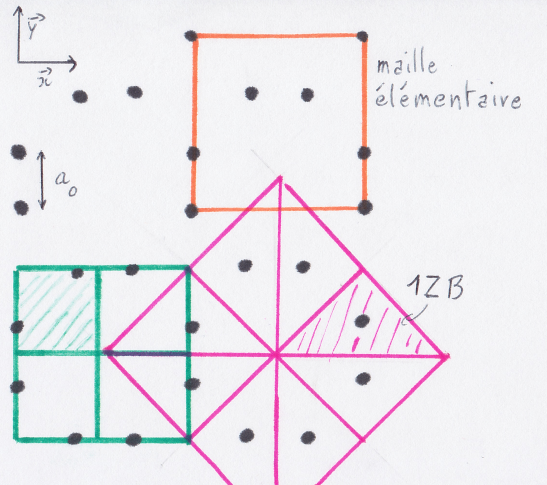
\includegraphics[width=8cm]{./pictures/mailles.png}
  \caption{Différentes mailles présentes dans le cristal}
  \label{fig:mailles}
\end{figure}




\begin{question}
  Préciser le motif associé à ce cristal : nombre d'atomes et position en fonction des vecteurs $\vv{a}$ et $\vv{b}$
\end{question}
Ce cristal présente un motif carré primitif contenant 4 atomes.
\begin{itemize}
\item (0,0) l'origine de la maille
\item (0,1/3)
\item (1/3,2/3)
\item (2/3,2/3)
\end{itemize}

  


\begin{question}
  Calculer l'aire de la maille unitaire, en fonction de $a_0$
\end{question}
L'aire de la maille unitaire est égale à celle de la maille élémentaire divisée par le nombre d'atomes dans cette dernière:
\begin{equation}\label{equ:SmailleU}
  A= \frac{a^2}{4} = {a_0}^2 \frac{9}{4}
\end{equation}

Nous retrouvons bien ce résultat avec les deux mailles unitaires que nous avions définis à la première question.

\begin{question}
  Calculer le nombre d'atomes par unité de surface. Application numérique en \si{\per\square\meter}.
\end{question}

Le nombre d'atomes par unité de surface est simplement l'inverse de la surface de la maille unitaire puisque cette dernière décrit la surface occupée par un atome, nous avons donc:
\[ \rho_a = \frac{4}{9{a_0}^2} = \SI{1,11e19}{\per\square\meter}\]

\begin{question}
  Exprimer les coordonnées des vecteurs du réseau réciproque $(\vv{a*}, \vv{b*})$, en fonction de $a_0$ dans le repère $Oxy$
\end{question}

Nous pouvons exprimer le réseau réciproque élémentaire, en posant $\delta_{i,j}$ l'opérateur de Kronecker, à partir de la relation suivantes:
\begin{equation}\label{equ:thRR}
  \vv{\imath}\cdot\vv{\jmath}^* = 2\pi\delta_{i,j}
\end{equation}

Si nous posons $\vv{a^*}=(\alpha,\beta)$ et $\vv{b*}=(\gamma,\eta)$, nous avons les relations suivantes:
\begin{align*}
  \vv{a^*}\cdot\vv{a}=2\pi \quad \Rightarrow \quad 3a_0\cdot \alpha = 2\pi \\
   \vv{a^*}\cdot\vv{b}=0 \quad \Rightarrow \quad 3a_0\cdot \beta = 0 \\
 \vv{b^*}\cdot\vv{b}=2\pi \quad \Rightarrow \quad 3a_0\cdot \eta = 2\pi \\
 \vv{b^*}\cdot\vv{a}=0 \quad \Rightarrow \quad 3a_0\cdot \gamma = 0 
\end{align*}
Un fois le système résolu, nous obtenons le réseau réciproque élémentaire de notre maille:
\begin{equation}\label{equ:RR}
  \vv{a^*} = \left(\frac{2\pi}{3 a_0},0\right) \qquad \vv{b^*} = \left(0,\frac{2\pi}{3a_0 }\right)
\end{equation}



\begin{question}
  Dessiner le réseau réciproque et le première zone de Brillouin
\end{question}

Pour la suite de l'exercice, nous négligeons complètement le fait que nous avons 4 atomes dans la maille, ce n'est pas un manque volonté, c'est simplement que l'auteur n'a pas
réussi à trouver une maille élémentaire satisfaisante afin de réaliser ces calculs. Nous avions supposé que nous pouvions réinsérer les noeuds de notre maille élémentaire dans
notre réseau réciproque en utilisant les résultats de la question~3. Cependant, en faisant ainsi, nous trouvons une première zone de Brillouin triangulaire rectangle ce qui nous empêche de résoudre la suite de l'exercice.


\begin{figure}[htb]
  \centering
  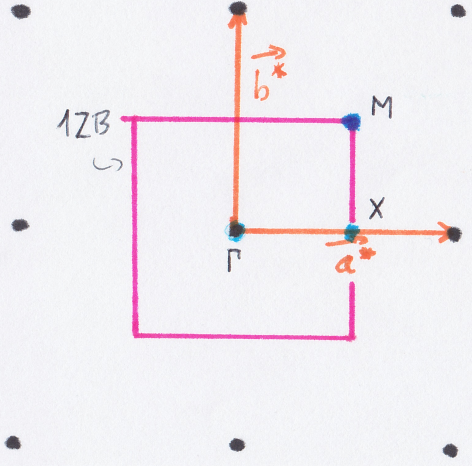
\includegraphics[width=9cm]{./pictures/1ZB.png}
  \caption{Réseau réciproque et première zone de Brillouin}
  \label{fig:RR}
\end{figure}

\begin{question}
  Dans la première zone de Brillouin, placer les points $\Gamma$ ,$X$ de coordonnées $(\frac{\pi}{a},0)$ et $M$ de coordonnées $(\frac{\pi}{a},\frac{\pi}{a})$.
\end{question}

\Question Si nous considérons maintenant une fonction de Bloch $\Psi_{c,k}$
\subquestion Les valeurs de $\vv{k}$ possibles dans la première zone de Brillouin sont les valeurs $\vv{k}=\frac{2\pi n}{L}$.
Ce résultat est obtenu quand nous considérons les conditions aux limites de la fonction de Bloch, nous considérons la limite sur la direction $\vv{x}$ mais la considération est identique pour la direction $\vv{y}$

\begin{align*}
  \Psi(x+L)& = \Psi(x) \quad \mbox{or} \quad \Psi(x)=u(x)e^{jk_x x} \\
  u(x+aN)e^{jk_x(x+Na)} &= u(x)e^{jk_xx} \quad   \mbox{avec}\quad u(x+a)=u(x)\\
  e^{jkNa} &= 1 \\
  k_xNa &= 2\pi n \quad n\in \mathbb{Z}
\end{align*}


\subquestion Nous pouvons ensuite calculer la densité d'états en vecteur d'onde. C'est l'inverse de l'espace occupé par un état, sachant qu'il y a deux états par vecteur d'onde, un pour les spin up et un pour les spin down.
\begin{equation}
  \rho_k = \frac{2 (Na)^2}{4\pi^2} = \frac{S}{2\pi^2}
\end{equation}

 \subquestion Pour déterminer le nombre d'états atomiques disponibles dans la première zone de Brillouin, il nous suffit de multiplier la densité d'états en vecteur d'onde avec la surface en vecteur d'ondes de la 1ere zone de Brillouin.
 \begin{equation}
   N_e = \rho_k*A_{1ZB} = \frac{(N a)^2}{2 \pi^2} \left(\frac{2\pi}{a}\right)^2 = 2N^2
 \end{equation}
 Le nombre d'états électronique est proportionnel au carré du nombre de répétitions de mailles dans une direction.


\partexo{Bandes d'énergie}
\begin{info}
  On suppose que l'énergie des électrons de conduction est représentée par :
  \begin{equation}\label{equ:enerelectron}
    E_c(\vv{k})= \alpha  - 2 \gamma \left( \cos(k_x a)  + \cos(k_y a)    \right)
  \end{equation}
\end{info}


\Question En prenant l'équation~\ref{equ:enerelectron} pour définir l'énergie des électrons de conduction, nous pouvons calculer l'énergie aux points caractéristiques de la maille en prenant $\alpha = \SI{2,5}{\eV}$ et $\gamma = \SI{0,5}{\eV}$:
\begin{itemize}
\item En $\Gamma$ ($\vv{k}=(0,0)$), nous avons: $E_{c\Gamma} = \alpha - 4\gamma= \SI{0,5}{\eV}$.
\item En $X$ ($\vv{k}=(\pi/a,0)$), nous avons: $E_{cX} = \alpha = \SI{2,5}{\eV}$ .
\item En $M$ ($\vv{k}= (\pi/a,\pi/a)$), nous avons: $E_{cM} = \alpha + 4\gamma = \SI{4,5}{\eV}$.
\end{itemize}

\Question En déterminant la ou les composantes de $\vv{k}$ qui varie ou varient en fonction de la direction dans laquelle nous nous déplaçons dans le cristal, nous pouvons réécrire la fonction $\vv{k}$ pour chaque direction:
\begin{itemize}
\item Sur la direction $\Gamma X$ ou $\Delta$, nous pouvons définir $\vv{k}$ en fonction de $x$ de la manière suivante:
  \begin{align*}
    \left[0,\frac{\pi}{a}\right] & \rightarrow \left[0,\frac{\pi}{a}\right]^2\\
    x                 & \mapsto    \vv{k} = (x,0) \\
  \end{align*}
  Nous pouvons donc définir la variation de l'énergie dans cette direction:
  \begin{equation}\label{equ:Delta}
    x\in\left[0,\frac{pi}{a}\right] \qquad E_{c\Delta} = \alpha - 2\gamma\left(1+\cos(ax)\right)
  \end{equation}

\item Sur la direction $\Gamma M$, nous pouvons définir $\vv{k}$ en fonction de $x$ de manière analogue:
  \begin{align*}
    \left[0,\frac{\pi}{a}\right] & \rightarrow \left[0,\frac{\pi}{a}\right]^2\\
    x                 & \mapsto    \vv{k} = (x,x) \\
  \end{align*}
  Nous pouvons donc définir la variation de l'énergie dans cette direction:
  \begin{equation}\label{equ:GammaX}
    x\in\left[0,\frac{pi}{a}\right] \quad E_{c\ \Gamma X} = \alpha - 4\gamma\cos(ax)
  \end{equation}

\item Sur la direction $XM$, nous pouvons aussi définir $\vv{k}$ en fonction de $x$:
  \begin{align*}
    \left[0,\frac{\pi}{a}\right] & \rightarrow \left[0,\frac{\pi}{a}\right]^2\\
    x                 & \mapsto    \vv{k} = (\frac{\pi}{a},x) \\
  \end{align*}
  Nous pouvons donc définir la variation de l'énergie dans cette direction:
  \begin{equation}\label{equ:XM}
    x\in\left[0,\frac{pi}{a}\right] \quad E_{c\ XM} = \alpha - 2\gamma(\cos(ax)-1)
  \end{equation}
\end{itemize}


Nous pouvons représenter l'évaluation de l'énergie en fonction de la position sur les principales directions, c'est que que nous faisons sur la figure

\begin{figure}[htb]
  \centering
%  \begin{pspicture}(-4,-1)(7.14,5)
%    \psline[showpoints=true, dotstyle=pentagon*](-3.14159,0)(0,0)(3.14159,0)(6.283185,0)
%    \psline[showpoints=true, dotstyle=pentagon*]{->}(0,0)(0,1)(0,2)(0,3)(0,4)(0,5)
%    %% M->Gamma
%    \def\EMG{x RadtoDeg cos -2 mul 2.5 add}
%    \psplot{-3.141592}{0}{\EMG}
%    \uput[d](-3,0){$M$}
%    %% Gamma -> X
%    \def\Delta{x RadtoDeg cos 1.5 sub neg}
%    \psplot{0}{3.141519}{\Delta}
%    \uput[d](0,0){$\Gamma$}
%    %% X -> M
%    \def\EXM{x 3.141519 sub RadtoDeg cos -1 mul 3.5 add}
%    \psplot{3.141519}{6.28318}{\EXM}
%    \uput[d](3.141592,0){$X$}
%    \uput[d](6.28318,0){$M$}
%    \rput(2,2){test}
%    
  %  \end{pspicture}
  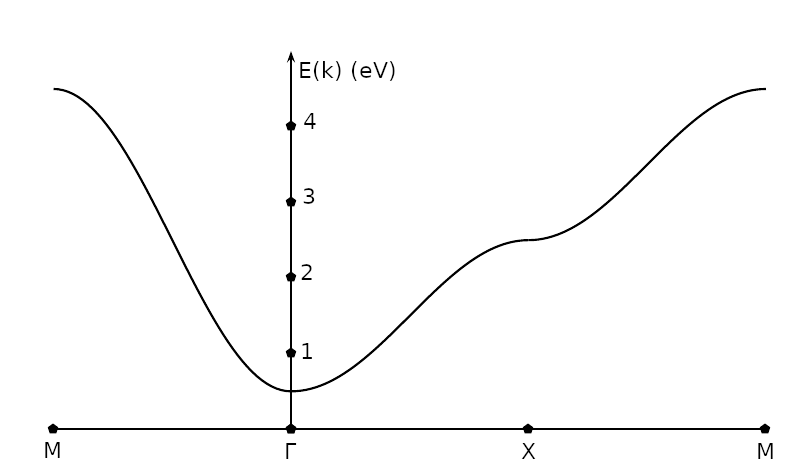
\includegraphics[width=0.6\textwidth]{./pictures/allure.png}
  \caption{Relation de dispersion}
  \label{fig:equdedispertion}
\end{figure}

\Question Nous pouvons maintenant exprimer l'énergie dans un voisinage de $\Gamma$ grâce à un développement limité:
\begin{equation}\label{equ:DL}
\mbox{pour $\vv{k}$ proche de $(0,0)$}\qquad E(k_x,k_y) = \alpha -4\gamma + 4a^2\gamma \left( {k_x}^2 + {k_y}^2 \right)
\end{equation}

Cette équation nous permet de définir la forme des lignes iso-énergie en fonction des directions des vecteurs
d'ondes. Puisque nous considérons des lignes iso-énergie, nous posons $E(k_x,k_y)=E_1$.

Nous avons alors la relation suivante:
\begin{equation}\label{equ:isoenergie}
  {k_x}^2 + {k_y}^2=\frac{E_1+4\gamma - \alpha}{4a^2\gamma}
\end{equation}
Cette relation correspond à l'équation d'un cercle, les lignes d'iso-énergie sont donc des cercles dans le domaines de
vecteurs d'ondes. L'énergie est donc \emph{isotrope}, ce qui nous permet de simplifier l'équation~\ref{equ:DL} en posant $k$ comme la distance entre le point que l'on considère et le centre de la maille ($k^2=k_x^2+k_y^2$):
\begin{equation}\label{equ:Energie}
  E(k)=\alpha-4\gamma+4a^2\gamma k^2
\end{equation}


\Question À partir de la relation~\ref{equ:Energie}, nous pouvons calculer la masse effective des électrons au voisinage de $\Gamma$.
\begin{align*}
  m^* &= \frac{\hbar^2}{\frac{\partial^2 E}{\partial k^2}} \\
    m^*& = \frac{\hbar^2}{8a^2\gamma}\\
    m^*& = {\SI{4,82e-32}{\kilogram}}\\
\end{align*}
Pour réaliser ce calcul, il faut faire attention à l'unité de $\gamma$, en effet, il est en $\si{\eV}$ , or nous avons réalisé le calcul dans le système international.

%%%%%%%%%%%%%%%%%%%%%%%%%%%%%%%%%%%%
%%%%%%%%%%%%%%%%%%%%%%%%%%%%%%%%%%%
\exercice{Méthode kp}

\Question Nous sommes en présence d'une équation aux valeurs propres qui peut s'écrire sous forme de matrice:
Nous posons:

\[ \hat{H}_{kp} =  \begin{bmatrix} E_G + \frac{\hbar^2 k^2}{2m_0} & Pk \\ Pk & \frac{\hbar^2 k^2}{2 m_0} \end{bmatrix} \qquad \ket{u_{n,k}} = \begin{bmatrix} C_1 \\ C_2 \end{bmatrix} \]

Nous avons alors l'équation suivante, avec $E$ un scalaire:
\begin{equation}\label{equ:evp_matrices}
  \hat{H} \ket{u_{n,k}} = E \ket{u_{n,k}} \quad \Leftrightarrow \quad \begin{bmatrix} E_G + \frac{\hbar^2 k^2}{2m_0} & Pk \\ Pk & \frac{\hbar^2 k^2}{2 m_0} \end{bmatrix} \times \begin{bmatrix} C_1 \\ C_2 \end{bmatrix} = E \begin{bmatrix} C_1 \\ C_2 \end{bmatrix}
\end{equation}

\Question Nous pouvons réécrire cette relation sous la forme $\left(\hat{H}-EI_2\right)\ket{u_{n,k}}=0$, or pour avoir une solution non-dégénérée à cette équation,
il faut trouver une énergie $E$ telle que l'image de la matrice $\hat{H}-EI_2$ soit 0, donc il faut en trouver un déterminant nul.
\begin{equation}\label{equ:determinant}
  \begin{vmatrix} E_G + \frac{\hbar^2 k^2}{2m_0} - E & Pk \\
    Pk & \frac{\hbar^2 k^2}{2 m_0} - E
  \end{vmatrix} = 0
  \quad \Leftrightarrow E^2-E\left(E_G + 2\left(\frac{\hbar^2 k^2}{2m_0}\right)\right) + \left(\frac{\hbar^2 k^2}{2m_0}\right)^2 + E_G \frac{\hbar^2k^2}{2m_0} - P^2 k^2 = 0
\end{equation}

\Question Nous calculons dans un premier temps le déterminant de ce plynôme du second degré en $E$, en posant: $P^2k^2 = E_P \frac{\hbar^2 k^2}{2 m_0}$
\begin{align*}
  \Delta &= \left( E_G + 2\left(\frac{\hbar^2 k^2}{2m_0}\right)\right)^2 -4\left(\frac{\hbar^2k^2}{2m_0}\right)^2 - 4E_G \frac{\hbar^2 k^2}{2m_0} + 4E_P\frac{\hbar^2 k^2}{2m_0} \\
  \Delta &= E_G^2 +4E_P \frac{\hbar^2 k^2}{2m_0} \\
\end{align*}

Nous pouvons donc maintenant exprimer les deux solutions du système~\ref{equ:determinant}:
\begin{equation}\label{equ:jaioublie}
  E_{c,v} = \frac{E_G}{2} + \frac{\hbar^2 k^2}{2m_0} \pm \frac{1}{2}\sqrt{E_G^2 + E_P \frac{\hbar^2k^2}{2 m_0}}
  \end{equation}

Les énergies $E_G$ et $E_P$ sont positives, tout comme le vecteur d'onde et la masse, la racine carrée présente dans l'équation~\ref{equ:jaioublie} est donc réelle, ce qui correspond à la réalite.
De plus, l'énergie de plus haut niveau semble correspondre à la bande de conduction et l'énergie la plus faible à la bande de valence, nous pouvons donc identifier les relations suivantes:
\begin{align}\label{equ:dispertion1}
  E_c &= \frac{E_G}{2} + \frac{\hbar^2 k^2}{2m_0} + \frac{E_G}{2}\sqrt{1 +4 \frac{E_P}{{E_G}^2} \frac{\hbar^2k^2}{2 m_0}}\\ \label{equ:dispertion2}
  E_v &= \frac{E_G}{2} + \frac{\hbar^2 k^2}{2m_0} - \frac{E_G}{2}\sqrt{1 +4 \frac{E_P}{{E_G}^2} \frac{\hbar^2k^2}{2 m_0}}
\end{align}

\Question Nous pouvons vérifier la validité de notre hypothèse précédente sur l'identité des bandes par un développement limité.
Une bande qui présente une courbure positive est une bande de valence là où une bande qui présente une courbure positive est une bande de conduction.

L'objectif de notre développement limité est d'éliminer la racine carrée dans les équations~\ref{equ:dispertion1}~et~\ref{equ:dispertion2}. Nous avons donc besoin
d'hypothèses sur les éléments présents dans cette racine. Nous supposons que $\frac{\hbar^2k^2}{2m_0} \ll \frac{E_G^2}{E_P}$ donc, nous avons $\frac{E_P}{E_G^2}\frac{\hbar^2k^2}{2m_0} \ll 1$ . Nous pouvons alors réaliser l'approximation suivante:
\begin{equation}\label{approximation}
  \sqrt{1+4\frac{E_P}{E_G^2} \frac{\hbar^2 k^2}{2 m_0}} \approx 1 + 2\frac{E_P}{E_G^2} \frac{\hbar^2 k^2}{2 m_0}
\end{equation}

En injectant la relation~\ref{approximation} dans les équations~\ref{equ:dispertion1}~et~\ref{equ:dispertion2}, nous obtenons de nouvelles expressions pour l'expression des énergies de conduction et de valence:
\begin{align}\label{equ:bande-intermédiaire1}
  E_c  &= E_G + \frac{\hbar^2 k^2}{2 m_0} \left(1+\frac{E_P}{E_G}\right) \\\label{equ:bande-intermédiaire2}
  E_v  &= \frac{\hbar^2 k^2}{2m_0} \left( 1-\frac{E_P}{E_G}\right)
\end{align}

Nous pouvons maintenant déterminer les courbure de chaque bande en calculant la dérivée seconde par rapport au vecteur d'onde $k$:
\begin{align} \label{equ:courbureC}
  \frac{\partial^2 E_c}{ \partial k^2} = \frac{\hbar}{m_0}\left( 1+\frac{E_P}{E_G}\right) \\\label{equ:courbureV}
  \frac{\partial^2 E_v}{ \partial k^2} = \frac{\hbar}{m_0}\left( 1- \frac{E_P}{E_G}\right)
\end{align}

Si nous considérons l'équation~\ref{equ:courbureC}, nous constatons que la courbure de la bande de conduction est bien positive.
Le signe de la courbure de la bande de valence est lui défini par le rapport $E_P/E_G$ dans l'équation~\ref{equ:courbureV}. Cette courbure est négative
si et seulement si $E_P>E_G$. Or on nous donne plus loin $E_P = \SI{16,0}{\eV}$ et $E_G\in [0,235;1,424]\si{\eV}$ donc nous vérifions cette hypothèse.

\Question En utilisant la notation de la masse effective, nous avons vu dans le cours que l'équation de dispersion de la bande de conduction pouvait s'écrire de la manière suivante:
\begin{equation}\label{equ:thEquDispertion}
  E(k) = E_G +\frac{k^2 \hbar^2}{2 m_e^*}
\end{equation}

\Question En prenant les équations~\ref{equ:bande-intermédiaire1}~et~\ref{equ:thEquDispertion}, nous pouvons identifier la masse effective:
\begin{equation}\label{equ:me}
  m_e^* =\frac{m_0}{1+\frac{E_P}{E_G}}
\end{equation}

\begin{table}[htb]
  \begin{equation*}
    \begin{array}{|c||c|c|c|c|c|}
      \hline
      \mbox{Paramètre} & E_G\ (\si{\eV}) & \Delta_{so}\ (\si{\eV}) & m_{hh}^* \ (m_0) & m_{lh}^* \ (m_0) & m_{so}^* \ (m_0) \\\hline
      \mbox{InSb}      & \num{0,235}     &  \num{0,81}            & \num{0,38}      & \num{0,015}     & \num{0,011}     \\\hline
      \mbox{InAs}      & \num{0,417}     &  \num{0,39}            & \num{0,41}      & \num{0,027}     & \num{0,014}     \\\hline
      \mbox{InP}       & \num{1,424}     &  \num{0,108}           & \num{0,78}      & \num{0,11}      & \num{0,021}     \\\hline
    \end{array}
  \end{equation*}
  \caption{Paramètres de structure de bande pour InSb, InAs et InP}
  \label{tab:donnes}
\end{table}

\Question À partir des données du tableau~\ref{tab:donnes}, et en prenant $E_P=\SI{16,0}{\eV}$, nous pouvons calculer les masses effectives de trois semi-conducteurs à gap direct en utilisant la formule~\ref{equ:me}:
\begin{description} 
\item{InSb: } $m_{e\ InSb}^* = \num{0,0145}\ m_0 = \SI{1,318e-32}{\kilogram}$
\item{InAs: } $m_{e\ InAs}^* = \num{0,0254}\ m_0 = \SI{2,314e-32}{\kilogram}$
\item{InP: } $m_{e\ InP}^* = \num{0,0817}\ m_0 = \SI{7,445e-32}{\kilogram}$
\end{description}

Le tableau~\ref{tab:donnes} ne nous permet pas de comparer nos résultats avec des mesures expérimentales.


\Question cf figure~\ref{fig:allureED}
\begin{figure}[htb]
  \centering
  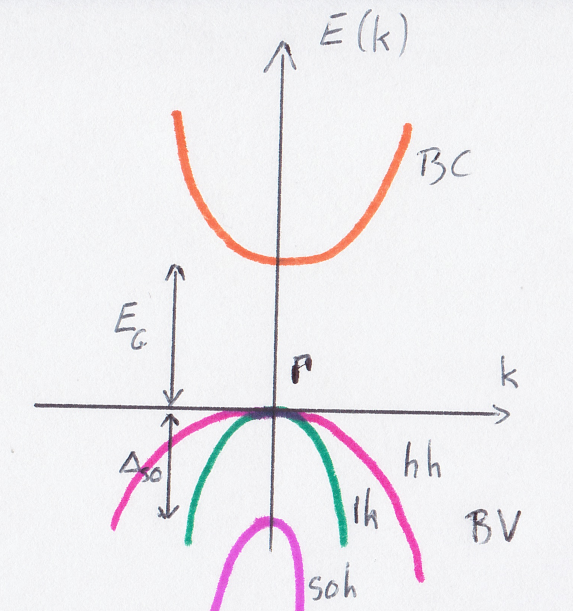
\includegraphics[width=7cm]{./pictures/bandes.png}
  \caption{Allure de la relation de dispertion en $\Gamma$ pour un semi-conducteur à gap direct}
  \label{fig:allureED}
\end{figure}




\Question Si nous considérons l'expression de $E_v$ de l'équation~\ref{equ:bande-intermédiaire2}, nous pouvons la comparer à une relation de dispertion isotrope parabolique de bande de valence pour les trous lourds ($hh$ pour \emph{heavy hole}) et les trous légers ($lh$ our \emph{light holes}):
\begin{equation}\label{equ:thDispertionValence}
  E_{v\ th} = -\frac{k^2 \hbar^2}{2 m_h^*} \qquad mbox{avec }m_h^* =\left\{\begin{matrix} m_{hh}^* \\ m_{lh}^*\end{matrix}\right.
\end{equation}

Par identification, nous obtenons une nouvelle équation pour les masses équivalentes des trous:
\begin{equation}\label{equ:met}
  m_h^* = \frac{m_0}{\frac{E_P}{E_G} -1}
\end{equation}

Nous pouvons alors appliquer les données du tableau~\ref{tab:donnes}:
\begin{description}
\item{InSb} $m_{h\ InSb}^* = \num{0,0149}\ m_0 = \SI{1,36e-32}{\kilogram}$. Ce résultat correspond, à l'approximation du nombre de chiffres significatifs près à la masse relative du trou léger pour ce semi-conducteur. 
\item{InAs} $m_{h\ InAs}^* = \num{0,0267}\ m_0 = \SI{2,44e-32}{\kilogram}$. Encore une fois, ce résultat correspond à un trou léger
\item{InP} $m_{h\ InP}^* = \num{0,097}\ m_0 = \SI{8,90e-32}{\kilogram}$. Ce calcul s'éloigne légèrement des données du tableau~\ref{tab:donnes} pour un trou léger, nous notons un écart absolu de 12\%. Cependant ce résultat ne correspond pas à la mesure d'un trou lourd pour autant avec un écart absolu de 88\%.
\end{description}

\Question Nous pouvons conclure de nos résultats que c'est la bande des \emph{trous légers} qui est correctement représentée par cette méthode. Cependant, l'écart avec le dernier semi-conducteur (InP) nous mène à croire que cette méthode fonctionne uniquement pour des énergies de gap suffisamment petites. Nous pouvons lier cet écart à l'hypothèse que nous avons posé:$\frac{\hbar^2k^2}{2m_0} \ll \frac{E_G^2}{E_P}$, cette hypothèse est levée pour de grandes énergies de gap.  
  






\end{document}

% LocalWords:  Hermitiques Schrödinger Hermitique iso-énergie
